\documentclass[a4paper,12pt]{article}

\usepackage[utf8]{inputenc}
\usepackage[russian]{babel}
\usepackage[top=2cm, bottom=2cm, left=2cm, right=2cm]{geometry}
\usepackage{amsmath, amsfonts, amssymb}
\usepackage{graphicx}
\usepackage{booktabs}
\usepackage{float}
\usepackage{caption}

\begin{document}
	
	\begin{center}
		\textbf{\Large Отчет по заданию № 1}
	\end{center}
	
	\vspace{0.5em}
	\noindent \textbf{Выполнила:} Оплаканская А.М., группа 26152. \\
	\textbf{Вариант 14.}
	
	\vspace{1em}
	\noindent \textbf{Описание задания:} В качестве базиса полиномиального пространства использовались полиномы Лежандра $P_j(\varepsilon)$ ($j = 0, \dots, N$). Для реализации численного решения переопределенной СЛАУ использовались: метод Нормальных Уравнений (НУ) с факторизацией Холецкого и QR-алгоритм на основе метода вращений Гивенса с выбором главного элемента по столбцам. Программа написана на языке \textbf{Rust}.
	
	\vspace{1em}
	\noindent \textbf{QR-разложение тестовой матрицы:} \\
	Для матрицы $A = \begin{pmatrix} 1 & 2 \\ 3 & 4 \\ 5 & 6 \end{pmatrix}$ методом вращений Гивенса получено разложение $A = Q \cdot R$:
	\[
	Q = \begin{pmatrix} 
		0.1690 & 0.8971 & 0.4082 \\ 
		0.5071 & 0.2760 & -0.8165 \\ 
		0.8452 & -0.3450 & 0.4082 
	\end{pmatrix}, \quad
	R = \begin{pmatrix} 
		5.9161 & 7.4374 \\ 
		0.0000 & 0.8281 \\ 
		0.0000 & 0.0000 
	\end{pmatrix}
	\]
	Проверка ортогональности $Q^T Q = I$ и равенства $Q R = A$ выполнена с машинной точностью.
	
	\vspace{1.5em}
	\noindent \textbf{Таблица 1.} Результаты численных экспериментов для данных  2
	\begin{table}[H]
		\centering
		\small
		\begin{tabular}{|c|c|c|c|c|c|c|}
			\hline
			$N$ & $\text{cond}_2(A^T A)$ & NRMSE  & Время , с & $\text{cond}_2(A)$ & NRMSE QR & Время QR, с \\ \hline
			0  & 1.00e+0  & 2.88e-1 & 0.00013 & 1.00e+0 & 2.88e-1 & 0.00031 \\ \hline
			1  & 3.06e+2  & 1.14e-2 & 0.00019 & 1.75e+1 & 1.14e-2 & 0.00063 \\ \hline
			2  & 8.25e+4  & 6.72e-4 & 0.00030 & 2.87e+2 & 6.72e-4 & 0.00105 \\ \hline
			3  & 3.21e+7  & 6.69e-4 & 0.00027 & 5.67e+3 & 6.69e-4 & 0.00138 \\ \hline
			4  & 1.25e+10 & 6.66e-4 & 0.00036 & 1.12e+5 & 6.66e-4 & 0.00188 \\ \hline
			5  & 5.33e+12 & 4.41e-4 & 0.00026 & 2.31e+6 & 4.41e-4 & 0.00229 \\ \hline
			6  & $\infty$ & 2.51e-4 & 0.00027 & 4.75e+7 & 2.47e-4 & 0.00276 \\ \hline
			7  & $\infty$ & 2.39e-4 & 0.00025 & 1.00e+9 & 2.36e-4 & 0.00358 \\ \hline
			8  & $\infty$ & 2.99e-4 & 0.00046 & 2.10e+10& 2.03e-4 & 0.00382 \\ \hline
			9  & $\infty$ & & ---     & 4.50e+11& 1.80e-4 & 0.00454 \\ \hline
			10 & $\infty$ & & ---     & 9.50e+12& 1.67e-4 & 0.00504 \\ \hline
		\end{tabular}
	\end{table}
	
	\noindent \textbf{Таблица 2.} Результаты численных экспериментов для данных  4
	\begin{table}[H]
		\centering
		\small
		\begin{tabular}{|c|c|c|c|c|c|c|}
			\hline
			$N$ & $\text{cond}_2(A^T A)$ & NRMSE  & Время , с & $\text{cond}_2(A)$ & NRMSE QR & Время QR, с \\ \hline
			0  & 1.00e+0  & 3.32e-1  & 0.00002 & 1.00e+0 & 3.32e-1  & 0.00006 \\ \hline
			1  & 1.92e+1  & 8.30e-2  & 0.00004 & 4.39e+0 & 8.30e-2  & 0.00012 \\ \hline
			2  & 4.00e+2  & 8.81e-15 & 0.00004 & 2.00e+1 & 2.15e-15 & 0.00019 \\ \hline
			3  & 1.07e+4  & 4.83e-14 & 0.00006 & 1.04e+2 & 2.17e-15 & 0.00027 \\ \hline
			4  & 3.10e+5  & 2.79e-13 & 0.00007 & 5.57e+2 & 1.99e-15 & 0.00037 \\ \hline
			5  & 9.36e+6  & 2.02e-12 & 0.00006 & 3.06e+3 & 2.04e-15 & 0.00040 \\ \hline
			6  & 2.88e+8  & 1.10e-11 & 0.00005 & 1.70e+4 & 2.05e-15 & 0.00047 \\ \hline
			7  & 9.03e+9  & 6.01e-11 & 0.00005 & 9.50e+4 & 2.03e-15 & 0.00060 \\ \hline
			8  & 2.86e+11 & 3.29e-10 & 0.00010 & 5.34e+5 & 1.93e-15 & 0.00078 \\ \hline
			9  & 9.12e+12 & 1.80e-9  & 0.00012 & 3.02e+6 & 2.05e-15 & 0.00102 \\ \hline
			10 & 2.97e+14 & 1.01e-8  & 0.00019 & 1.71e+7 & 2.09e-15 & 0.00117 \\ \hline
		\end{tabular}
	\end{table}
	
	\newpage
	
	\noindent \textbf{Таблица 3.} Результаты численных экспериментов для данных  5
	\begin{table}[H]
		\centering
		\small
		\begin{tabular}{|c|c|c|c|c|c|c|}
			\hline
			$N$ & $\text{cond}_2(A^T A)$ & NRMSE  & Время , с & $\text{cond}_2(A)$ & NRMSE QR & Время QR, с \\ \hline
			0  & 1.00e+0  & 2.94e-1  & 0.00003 & 1.00e+0 & 2.94e-1  & 0.00005 \\ \hline
			1  & 1.92e+1  & 2.76e-2  & 0.00004 & 4.39e+0 & 2.76e-2  & 0.00011 \\ \hline
			2  & 4.00e+2  & 2.32e-3  & 0.00006 & 2.00e+1 & 2.32e-3  & 0.00017 \\ \hline
			3  & 1.07e+4  & 1.46e-4  & 0.00006 & 1.04e+2 & 1.46e-4  & 0.00024 \\ \hline
			4  & 3.10e+5  & 7.32e-6  & 0.00009 & 5.57e+2 & 7.32e-6  & 0.00032 \\ \hline
			5  & 9.36e+6  & 3.06e-7  & 0.00007 & 3.06e+3 & 3.06e-7  & 0.00040 \\ \hline
			6  & 2.88e+8  & 1.09e-8  & 0.00007 & 1.70e+4 & 1.09e-8  & 0.00044 \\ \hline
			7  & 9.03e+9  & 3.43e-10 & 0.00007 & 9.50e+4 & 3.43e-10 & 0.00050 \\ \hline
			8  & 2.86e+11 & 8.53e-11 & 0.00013 & 5.34e+5 & 9.54e-12 & 0.00066 \\ \hline
			9  & 9.12e+12 & 4.39e-10 & 0.00020 & 3.02e+6 & 2.39e-13 & 0.00090 \\ \hline
			10 & 2.97e+14 & 2.32e-9  & 0.00018 & 1.71e+7 & 5.52e-15 & 0.00091 \\ \hline
		\end{tabular}
	\end{table}
	
	\begin{figure}[H]
		\centering
		% Файл plot_result.png должен лежать в той же папке
		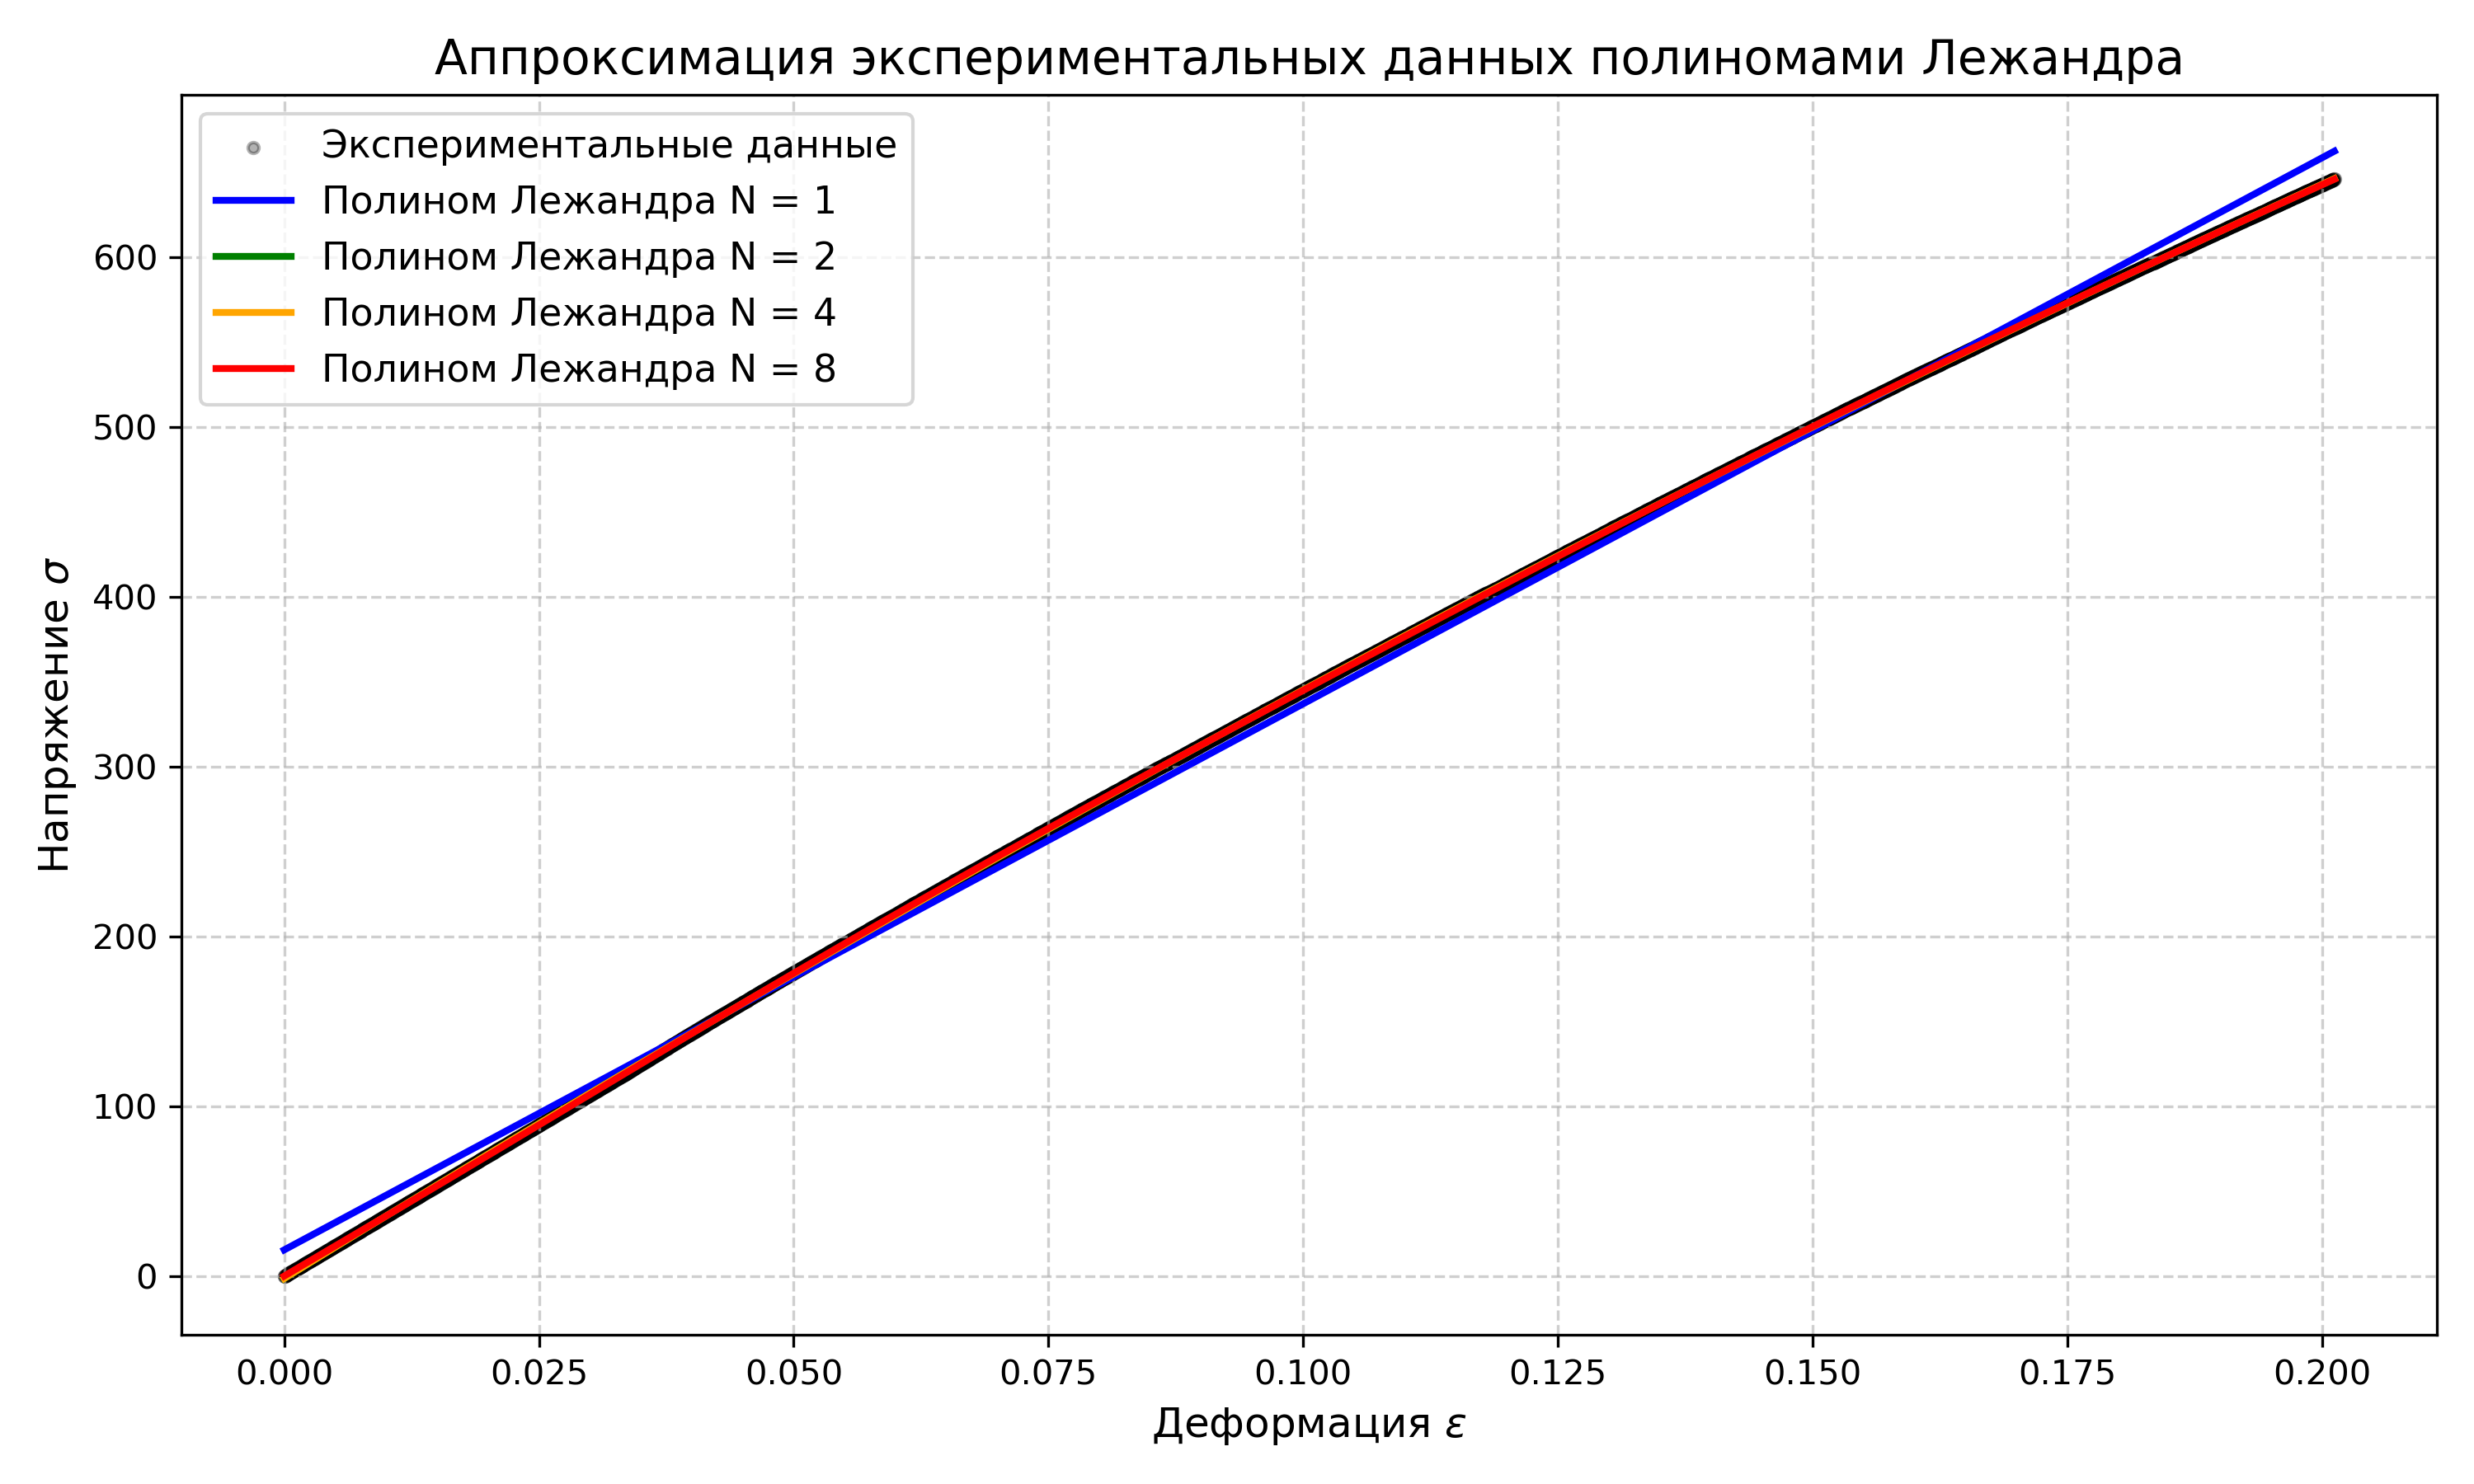
\includegraphics[width=0.88\textwidth]{plot_result.png}
		\caption{График экспериментальных данных и их аппроксимации полиномами Лежандра}
	\end{figure}
	
	\vspace{1em}
	\noindent \textbf{Выводы:}
	
	\begin{enumerate}
		\item \textbf{Сравнение чисел обусловленности:} Численные рачеты подтвердили фундаментальное теоретическое соотношение $\text{cond}_2(A^T A) = [\text{cond}_2(A)]^2$. В силу квадратичного роста число обусловлености нормальной СЛАУ быстро достигает ($10^{16}$). Для данных 2 уже при $N \ge 6$ наблюдается $\text{cond}_2(A^T A) = \infty$, а при $N = 9, 10$ матрица теряет численную положительную определенность, приводя к остановке метода Холецкого. Метод QR работает с матрицей $A$, где обусловленность сохраняется в допустимых пределах ($\sim 10^7 - 10^{12}$).
		
		\item \textbf{Характер убывания погрешности:} С увеличением степени полинома $N$ погрешность аппроксимации NRMSE монотонно уменьшается. Для данных 4 уже при $N = 2$ погрешность достигает ($\sim 10^{-15}$), это говорит о строго квадратичной природе исходной зависимости. Для гладких данных 5 наблюдается непрерывное экспоненциальное убывание ошибки вплоть до $N = 10$.
		
		\item \textbf{Сравнение точности методов НУ и QR:} 
		При малых степенях $N \le 4$ оба метода показывають идентичную точность. При больших степенях $N \ge 6$ метод НУ начинает страдать от критической потери точности из-за ошибок округления: в Таблицах 2 и 3 видно, что погрешность НУ начинает \textbf{возрастать} ( и еще на данных 4 ухудшается с $10^{-15}$ до $10^{-8}$). В то же время, метод вращений Гивенса демонстрирует численную устойчивость, удерживая погрешность на уровне $10^{-15}$.
	\end{enumerate}
	
\end{document}